\documentclass[10pt,a4paper,notitlepage, twocolumn]{article}
\usepackage[utf8]{inputenc}
\usepackage{amsmath}
\usepackage{amsfonts}
\usepackage{graphicx}
\usepackage{amssymb}
\usepackage{float}
\usepackage{listings}
\usepackage{lipsum}

\author{Nathaniel Forde}
\title{Decision and Expected Value}
\begin{document}


\section*{The Workhorse}
There is an algorithm beloved by bureaucrats, the unsung hero of administrators and accountants. An algorithm  both ubiquitous and under appreciated. It's pivotal for nearly every project and informs the actions of tech giants and policy makers the world over. It is only mildly hyperbolic to say that understanding this formula unlocks wealth and power. It lies at the heart of online A/B testing, all policy analysis, sound business strategy and poker play. In words: The expected financial value of a repeated process is just the sum of the possible outcomes weighted by their probabilities. 
$$ EV(O)_{p} = p_{1}v(o_{1}) + p_{2}v(o_{2}) + ... + p_{k}v(o_{k}) $$
Outcomes can vary from deals of cards, to customer transactions and election results. \footnote{In the jargon $O$ is a random variable which can be realised as any of the outcomes  $ o_{j} :  1 \leq j \leq k$} But aside from the mercenary possibilities, the formula merits your attention for the light it sheds on the puzzling topic of probabilities. With real stakes on the line, the meaning of probability is not an idle concern. The formula for expected value is glossed as one which governs rational action. Yet, statistics are tortured and probabilities are abused to fit policy prescriptions and rubber stamp decisions. False precision of risk models is common place, often callous and occasionally insidious. Nevertheless the rule has an enduring appeal that is worth the work it takes to understand it. 

\subsubsection*{Two sides of a Coin}
Probability has a dual aspect. On one reading it refers to the long run tendency of a random process, on another the probability is construed as the degree of belief in the an outcome. On the first interpretation the probability is a distribution with certain fixed theoretical characteristics (e.g. a uniform probability distribution is assumed in the roll of die, where all outcomes are equally likely). On the second reading the characteristics of the probability distribution are learned from the data. These approaches are united by the Law of Large numbers which states that as the size of our sample increases our sample average will converge to the expected realisation of the theoretical process.
$$  \frac{1}{N} \sum_{i = 1}^{N} O_{i} \text{ converges to }  E(O) \text{ as } N \text{ approaches } \infty $$ 
In the below plot we have stipulated a Poisson distribution with a mean of 4.5 and can see three examples of how consecutive averaging from the increasing sample sizes results in a closer and closer convergence to the population mean.

\begin{figure}[H]
  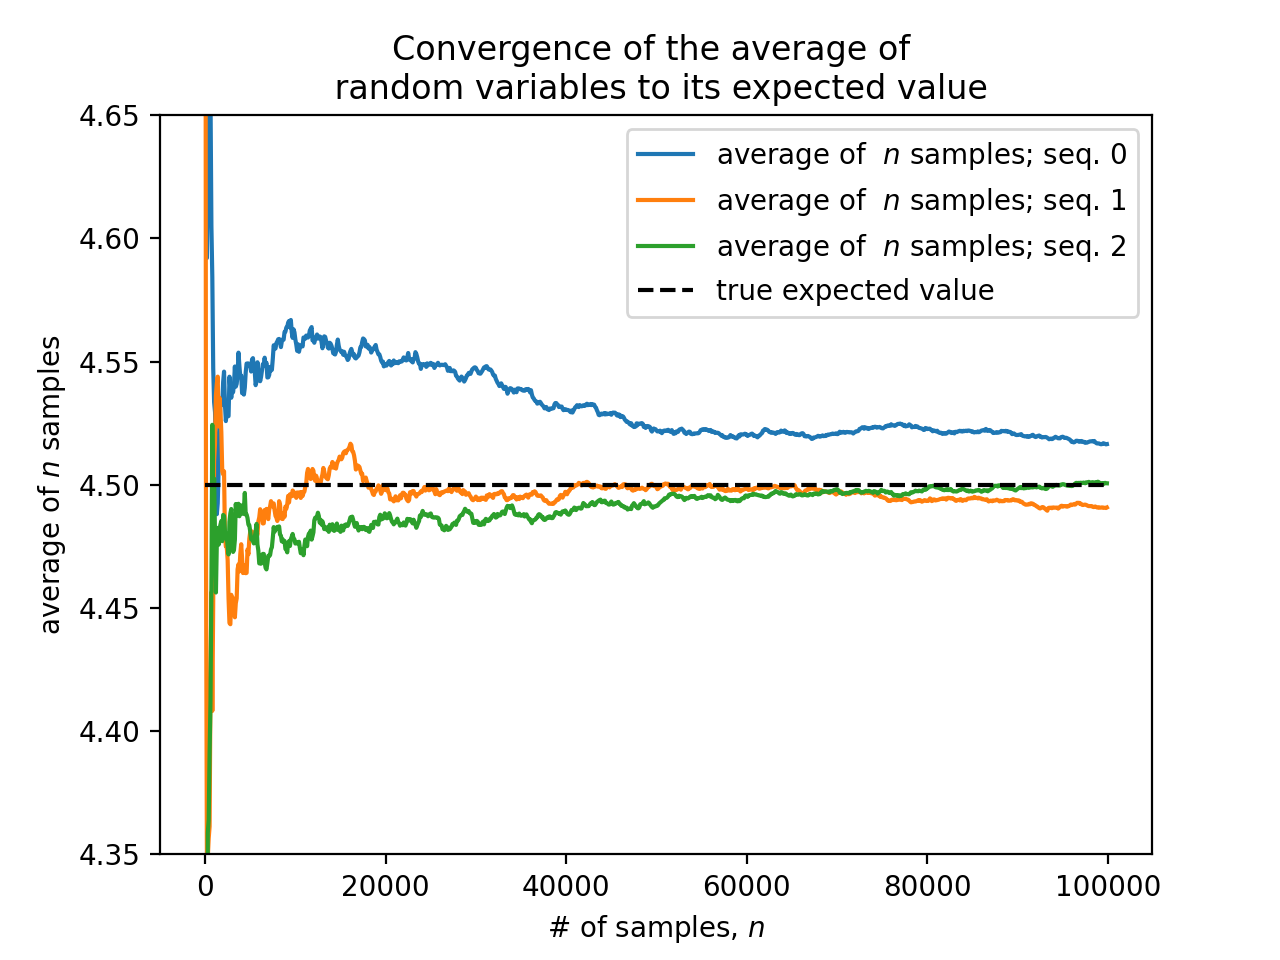
\includegraphics[width=\linewidth]{./Plots/convergence_of_law_of_large_numbers.png}
\end{figure}
\noindent  This is fundamental to the long-run tendency interpretation of probability. Given a game with fixed and fair odds we see that repeated play will converge because of characteristics which govern the process. Dice are the paradigm example.  In the wild we never know the characteristics which cause the spread of outcomes, but such is the influence of gambling on the consideration of probability, that the default assumes a stable pattern in the generating process. Partially this is pragmatic. The maths are more tractable if we can assume one well behaved underlying process. The results are compelling. The Normal (Bell Curve) distribution, the Poisson distribution the Bernoulli distribution (to name a few) are all rightly famous. Their shapes are characteristics of innumerable random processes. But the paradigm clouds the fact that in practice we start on the left side of the law of large numbers (with samples) and we often start with small numbers. 
\begin{figure}[H]
  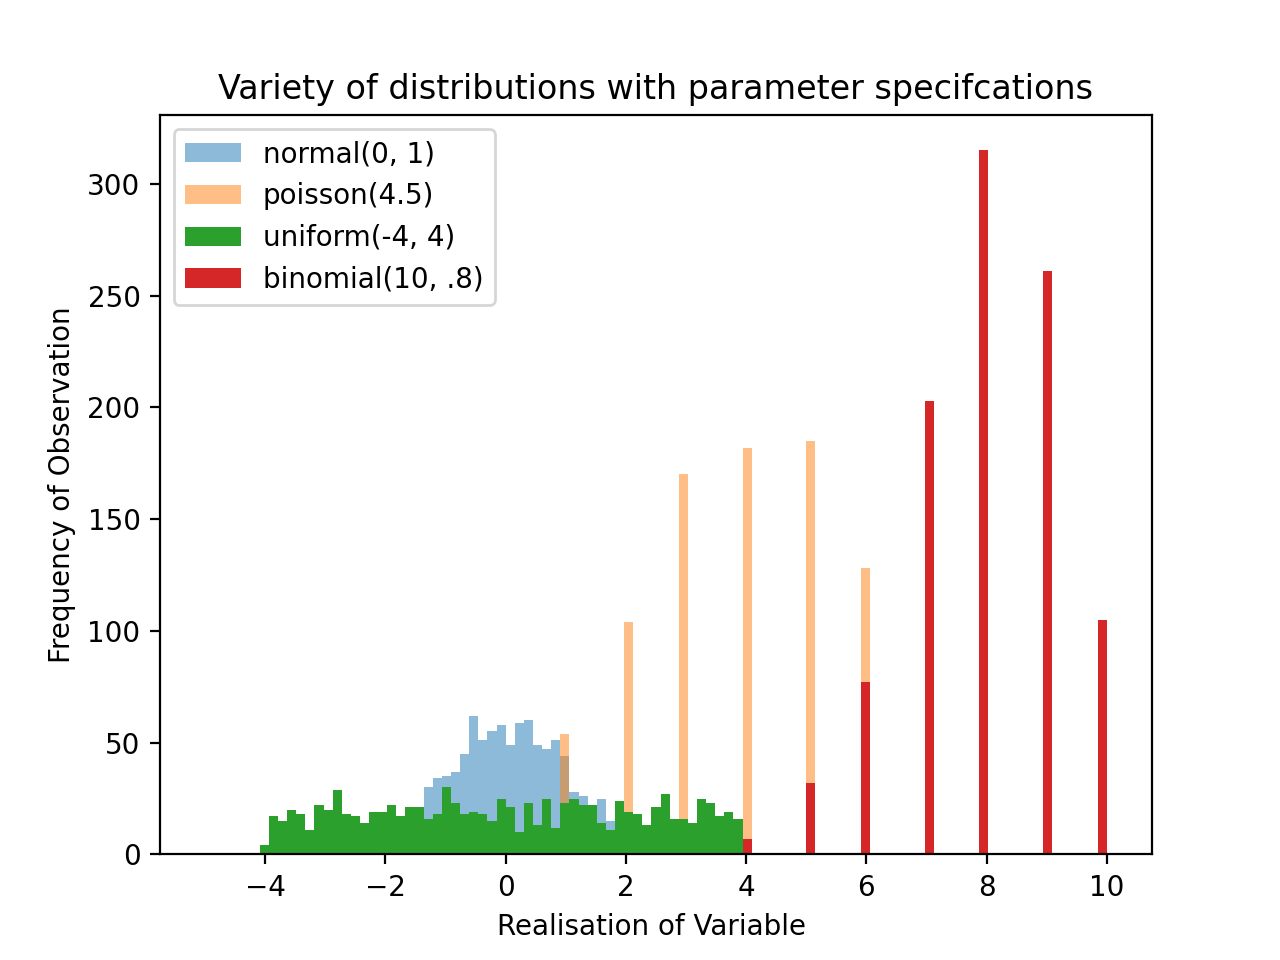
\includegraphics[width=\linewidth]{./Plots/variety_of_distributions.png}
\end{figure}
Well behaved probability distributions are rare beasts; a tiny fraction of the world's arbitrary menagerie. The fundamental question in probability is not whether probability is a measure of belief or frequency - it is whether we can safely assume that the underlying process adheres to a known model? If so, we can rely on the structure of the model's theoretical distribution to inform inference. If not we are better learning from the data - trusting to the sampling distribution and worst scenario planning.

\subsubsection*{Models, Errors and Expectations}
When your only tool is a hammer, then everything is a nail. When one model won't do, use two. This is roughly the approach adopted when models fail. The problem is especially vivid in time-series forecasts; projected death rates, body counts and stock prices are all subject to sudden shocks. A basic regression model has following form:

$$ Y = const + \beta X + \epsilon $$

\noindent where $\epsilon$ is a random variable representing the error. A modest notational device for disaster. While $const, \beta$ are parameters estimated by an optimisation process to ensure the equation fits the data as neatly as possible, assuming some degree of error. In the below graph we have a series characterised by change. After the first shock we can refit the model so that the line tracks well with the evolving data. After the second shock we try another refit, but the range the and variance of the data makes our basic model a poor fit. This presents three examples of error in the modelling process: (i) forecasts fail for the reason that's it's also difficult to identify (in the moment) those changepoints in the data which reflect structural change, (ii)  the fundamental assumptions that go into the model are sound, but the parameters need be re-estimated based on the new data
\begin{figure}[H]
  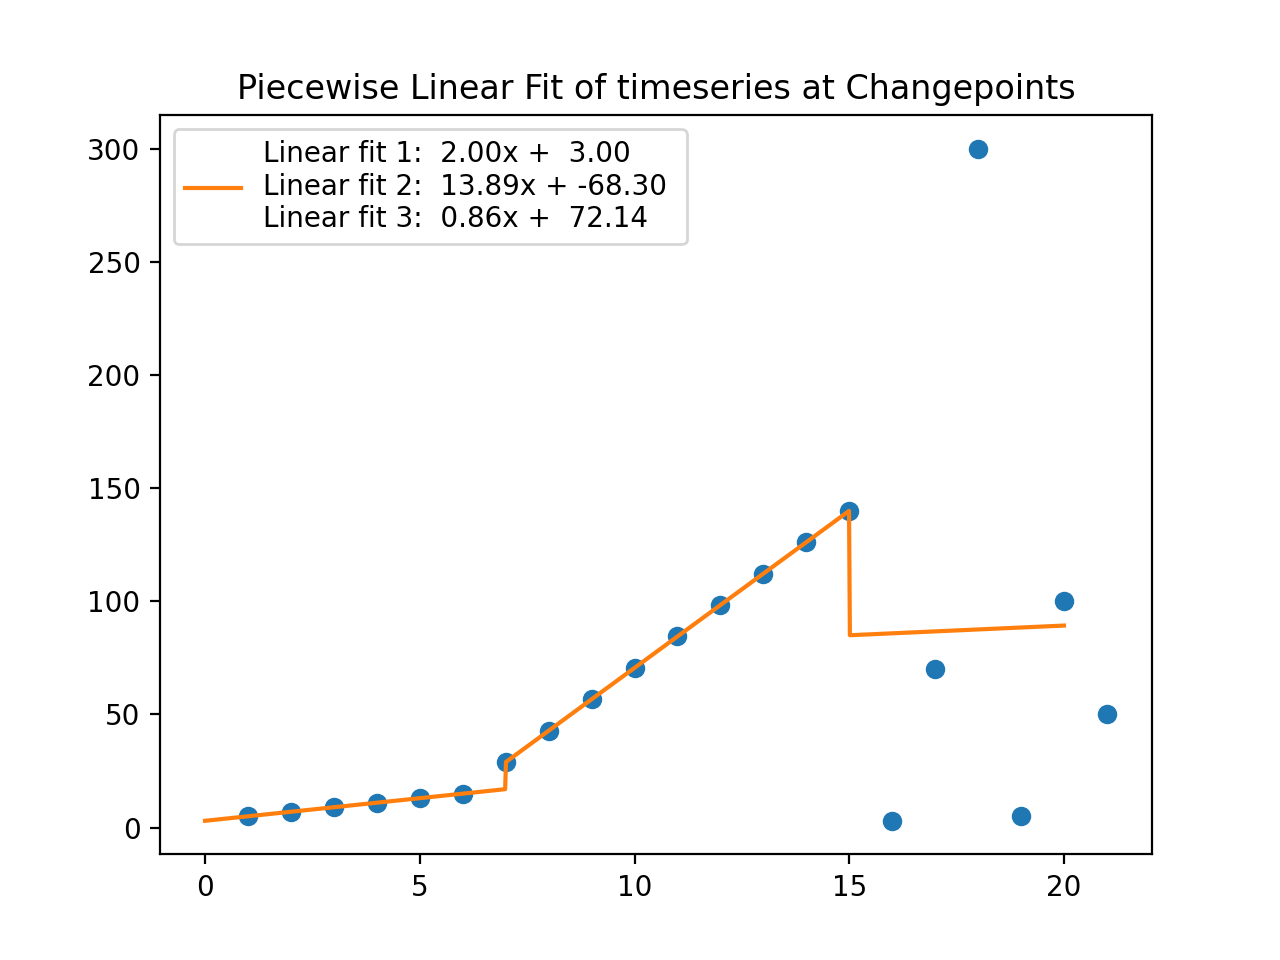
\includegraphics[width=\linewidth]{./Plots/piecewise_linear_fits.png}
\end{figure}
and (iii) the third linear model is simply a terrible match for the pattern in the data. In practice you never really know whether a new error stems from a misfit but appropriate model or an entirely inappropriate model. But as we increase our number of sample fits we hope to better approximate the true linear process (if any) generating the data. This warrants a note about errors. Imagine now that the data points on our previous graph are repeatedly re-speckled over the canvas. We can refit a new model for each set of scattered data points and each refit gives us a new sample values for $ const, \beta$. If the underlying data generating process is stable, then the parameter fits will converge to the characteristics of the stable process\footnote{The correct values of $const, \beta$. For example if the we're predicting height based on weight, our values for $const$ should be above 4.ft and the value for $\beta$ should be calibrated to make up the average difference when multiplying the value for weight.} Our sample estimates will overshoot in some cases but on the whole the errors up and down will cancel each other out if the errors themselves are normally distributed and the expected realisation of the error $\epsilon$ term is 0. Forecasting with the expected parameters derived from our sampling distribution minimises our forecast errors because the fluctuations are stable about the centre. These are assumptions required for a process to exhibit the tendency of regression towards the mean. 

The code below builds two sampling distributions based on different underlying processes.  One in which the errors are independent, normally distributed around 0 the other in which the errors are correlated in a sine-wave like pattern, increasing and decreasing periodically. This is akin to difference between measuring error when predicting the heights of randomly sampled people versus predicting the sales volumes on randomly selected days of the week. A random sample of daily sales  risks clumping weekends together and skewing the expected values. No such risk exists when sampling from independent individuals. 

\begin{lstlisting}[language=Python]
### Build True Models
N = 100000
X = np.random.uniform(0, 20, N)
independent_err = 
np.random.normal(0, 10, N)
corr_err = 
np.random.uniform (0, 10) + 
np.sin(np.linspace(0, 10*np.pi, N)) + 
np.sin(np.linspace(0, 5*np.pi, N))**2 + 
np.sin(np.linspace(1, 6*np.pi, N))**2

Y_corr = -2 + 3.5 * X + corr_err

Y = -2 + 3.5 * X + independent_err

population = pd.DataFrame({'X': X,
 'Y': Y, 'Y_corr': Y_corr})

### Sample from Data 
### and build smaller models

fits = DataFrame(columns=['iid_const',
 'iid_beta', 'corr_const', 
 'corr_beta'])
 
for i in range(0, 10000):
    sample = population.sample(n=100, 
    replace=True)
    Y = sample['Y']; X = sample['X']
    Y_corr = sample['Y_corr']
    X = sm.add_constant(X)
    iid_model = sm.OLS(Y, X)
    results = iid_model.fit()
    corr_model = sm.OLS(Y_corr, X)
    results_2 = corr_model.fit()
    row = [results.params[0], 
    results.params[1],
    results_2.params[0], 
    results_2.params[1]]
    fits.loc[len(fits)] = row
    
fits.boxplot()
\end{lstlisting}


\begin{figure}[H]
  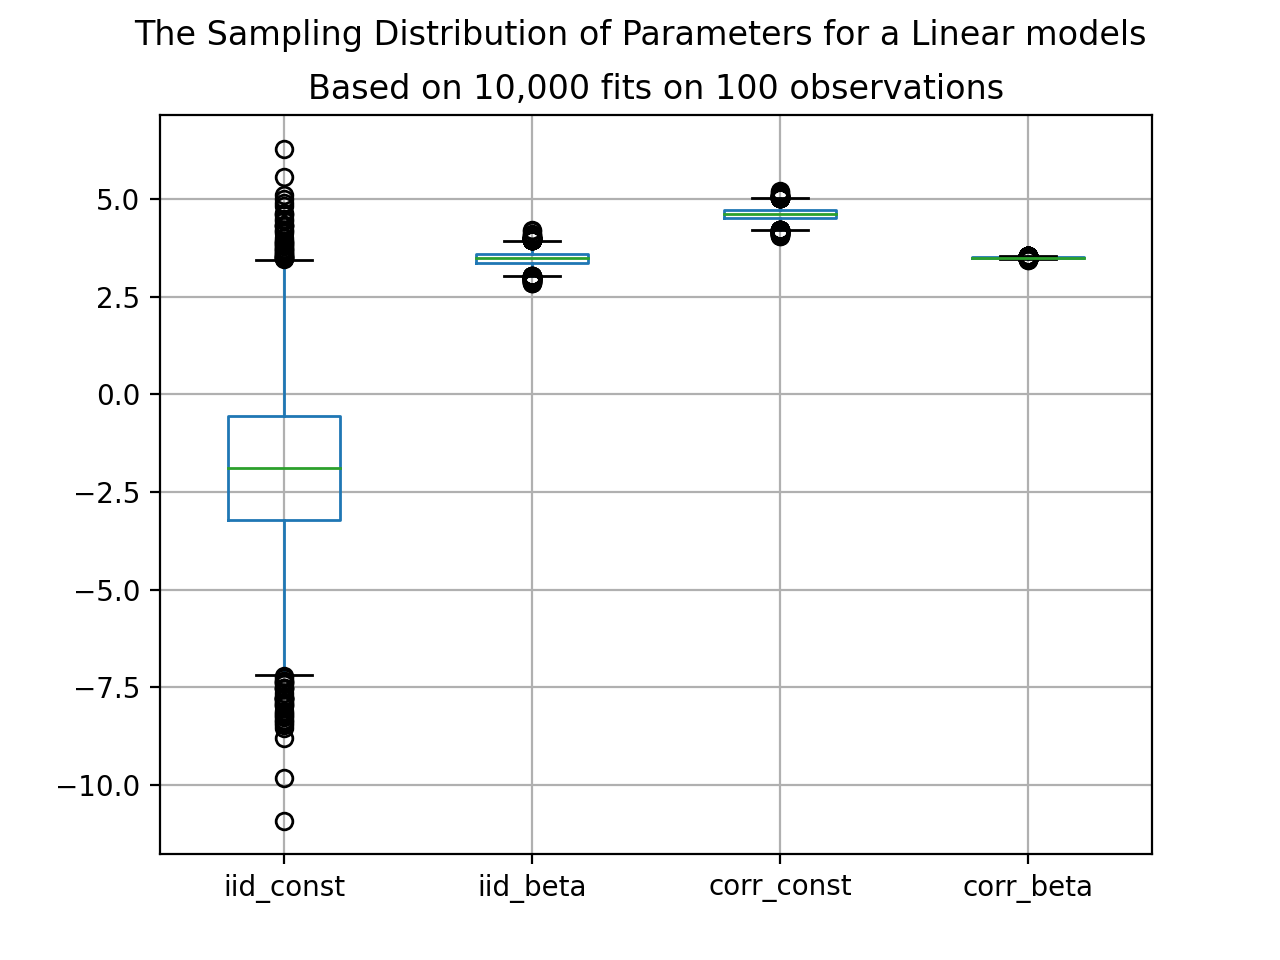
\includegraphics[width=\linewidth]{./Plots/distribution_of_beta1.png}
\end{figure}

In the case with independent errors the expected value for our parameter estimates match almost exactly the true values of the process. In the second model with correlated errors the parameter estimate for our constant is 4.9 which is significantly different from the true value of -2, and will lead to systematically skewed predictions.

\subsection*{Small World of the Model}
Prediction precedes probability in the order of analysis. Without a reliable regularity underwriting our observations, we interpret them as timorous noise. Only when there is a better than arbitrary correlation between $X, Y$ will we even think to ascribe a measurable probability to their association. Whether we view probabilities as a measure of credibility or frequency, the focus is always on a process which in reality reveals a pattern under repetition. We're loath to apply a probability model of any kind without some inductive evidence.
\newline 

\noindent So when does it make sense to use models? In what sense should expected values guide our action? These are questions which arise in any sustained investigation of a random process. If models are mere heuristics, from where do we pluck the values for $$p_{i} : 1 \leq i \leq k$$ in the formula $(EV)$. Models are deliberate simplifications of complexity, a toy version of the world. While recent innovations of in machine learning means that we can fit models with hundreds, thousands and even billions of parameters but this increase scale does not change fact that models are blind to all factors outside their samples. A good model predicts the variance in future data, in part, by ignoring the genuine complexity of reality. This is the only practical test that matters. If the prediction accuracy holds over successive periods we should become increasingly sure that the probabilities in our model are a good measure of risk. But we can never be certain the model holds over all successive periods and is robust to changes in external factors. We can however quantify the degree of uncertainty in the model by observing the spread of the sampling distribution. It's at this point that we can debate the finer points of statistical inference. 

\subsubsection*{Inference from Expected Frequency}
If you count the number heads in a series of successive coin flips, you'll arrive a proportion which characterises that process. If it's a fair coin roughly half of your sample will be heads. If the coin is weighted you might have as few as 0. This is the binomial distribution, and it really shine when you're trying to gauge fairness. If a process is biased, the distribution will be skewed. We can use this fact for inference. Consider a dispute over whether the game was rigged. 
$$ H_0 : \text{ proportion of heads } = 0.4  $$
$$ H_1 : \text{ proportion of heads } =  0.5 $$

\noindent Take $(H0)$ as given then if we observe a sequence $H, H, H, T, T$ consistent with $(H0)$ you might begin to think we're being hustled. The pattern of reasoning is straightforward (i) make some assumptions about the random process under investigation, (ii) tease out the consequences of these assumptions (iii) evaluate the incoming data to see if you need to revise your assumptions. 

\begin{figure}[H]
  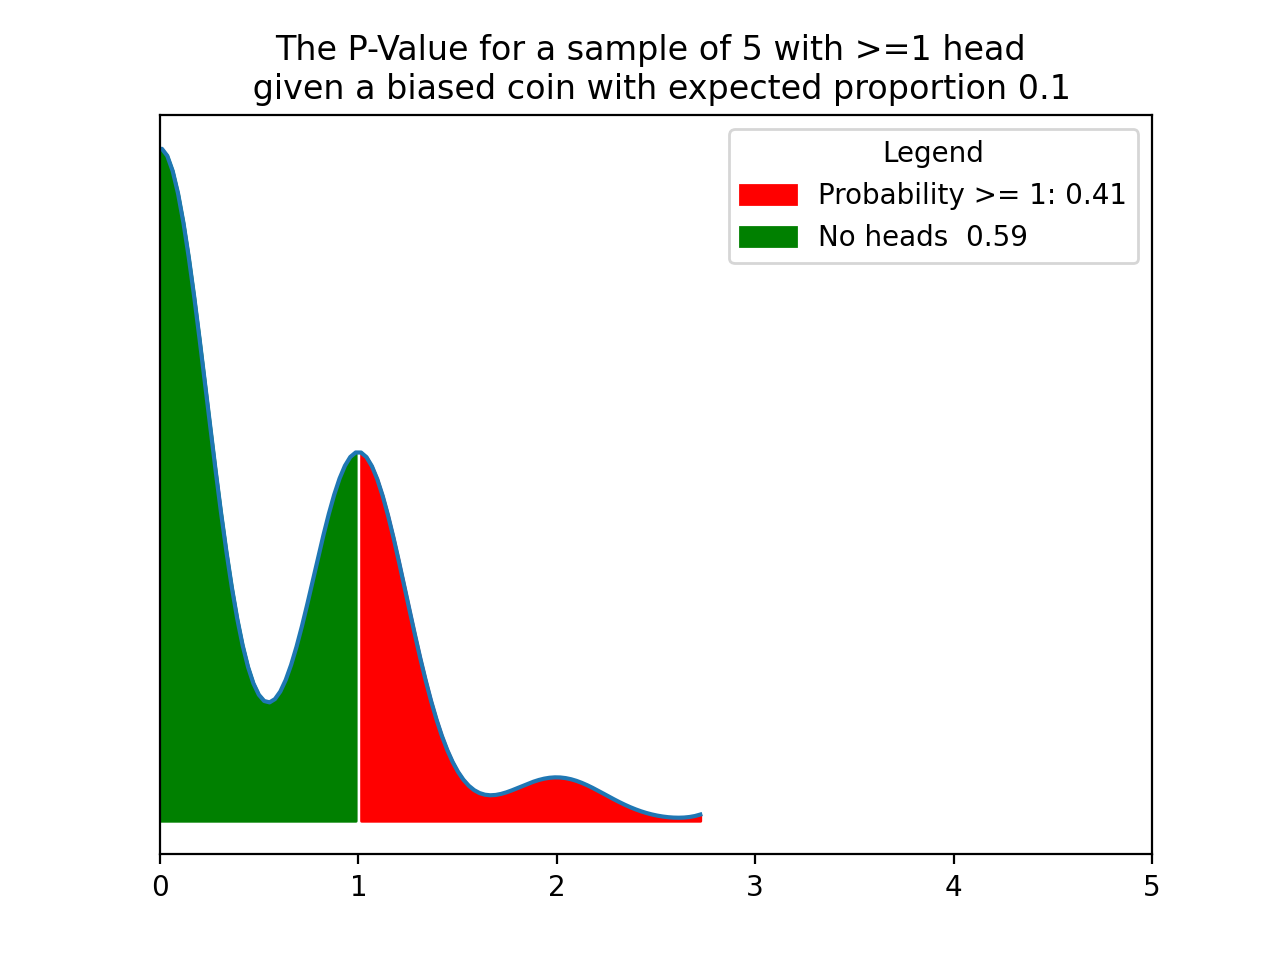
\includegraphics[width=\linewidth]{./Plots/binomial_test.png}
\end{figure}

In this instance there is significantly greater than the traditional 5\% chance of observing the above sequence so we do not have sufficient reason to reject $(H0)$, and should spend our money elsewhere. 

\subsubsection*{Inference from Prior Belief}
On the other hand if we instead use probability to simply calibrate our beliefs, then we should be more explicit in our assessment of $(H0), (H1)$. Let's assume that our prior beliefs about whether the game is rigged is 50/50. Then we evaluate the two hypothesis using Bayes's rule for incorporating our prior belief and the data. 

$$ \overset{posterior}{p(H_{i} | Data)} = \frac{\overset{prior}{p(H_{i})}\overset{liklihood}{p(Data | H_{i})}}{\sum_{i=1}^{i =K} p(Data | H_{i})p(H_i)}$$

where $ 1 \leq i \leq K$ spans the ways in which the data could have been realised. Then we have:

$$ \frac{p(H_1 | 3 in 5)}{p(H_{0} | 3 in 5)} = \frac{\frac{.5\cdot .31}{.5\cdot .31 + .5 \cdot .23}}{\frac{.5\cdot .23}{.5\cdot .31 + .5 \cdot .23}} = \frac{.57}{.42} $$

which would lead us to infer that the die was fair. 

\subsubsection*{The Art of Inference}
Neither analysis ends with these calculations, both would continue to probe the limits of each hypothesis. We'd have to consider things like sample size and sensitivity testing, model performance and cost of errors. The point is just that there are reasons for dispute. This is example shows the heart of the conflict between the dual aspect of probability. There is enough latitude in the manner in which we set up a probability model that the mathematics can yield apparently inconsistent results. The frequentist evaluation of our biased coin is very sensitive to the choice of hypotheses, while the Bayesian approach is influenced by the choice of prior. Why set up a significance test against assumed cheating rather than assumed fairness? Why attribute equal weight to both hypotheses? Both approaches come with baggage. 



\end{document}

